\section{}

\textbf{Tiempo de lectura:} \{s20-reading-time\}

Como ya hemos comentado, un sistema de archivos suele estar compuesto de
varios niveles diferentes. En la
\hyperref[fig-estructura-sistema-de-archivos]{???} se muestra un ejemplo
de la estructura de un sistema de archivos diseñado en niveles. Cada
nivel utiliza las funciones de los niveles inferiores y proporciona
nuevas funciones a los niveles superiores. El papel de cada uno de estos
niveles fue descrito en el
\hyperref[_estructura_de_un_sistema_de_archivos]{???}. Mientras que las
estructuras de metadatos utilizadas, tanto en la memoria como en disco,
fueron tratadas brevemente en el
\hyperref[_estructuras_de_metadatos_en_disco]{???} y en el
\hyperref[_estructuras_de_metadatos_en_memoria]{???}.

A continuación, vamos a profundizar aún más en las estructuras y
operaciones utilizadas para implementar los sistemas de archivos

\section{Implementación de
directorios}\label{_implementaciuxf3n_de_directorios}

Cada directorio suele contener una estructura de datos que relaciona el
nombre de cada archivo que contiene con el identificador de su
\textbf{FCB}. Dicho identificador permite localizar el FCB en la
\textbf{tabla de contenidos del volumen}, que contiene el resto de los
atributos del archivo.

En esta sección vamos a estudiar las formas más comunes de implementar
la estructura de datos de un directorio.

\subsection{Lista lineal}\label{_lista_lineal}

El método más simple para implementar un directorio consiste en utilizar
una lista lineal o vector de nombres de archivos e identificadores del
\textbf{FCB}.

Las acciones a realizar, para implementar cada una de las posibles
operaciones sobre el directorio, serían:

\begin{itemize}
\item
  \textbf{Crear un archivo}. Primero se explora el directorio para estar
  seguros de que no haya ningún archivo con el mismo nombre. Después se
  añade una nueva entrada al final del directorio.
\item
  \textbf{Borrar un archivo}. Primero se explora la lista en busca del
  archivo especificado y, una vez localizada, se libera la entrada
  correspondiente. Para reutilizar la entrada del directorio tenemos
  diversas alternativas:

  \begin{itemize}
  \item
    Se puede marcar la entrada como no utilizada. Para eso se puede
    emplear un nombre especial o utilizar algún campo adicional ---a
    parte de nombre de archivo e identificador del \textbf{FCB}--- que
    se haya añadido a la entrada con ese propósito.
  \item
    Insertar un puntero a la entrada en una lista de entradas libres,
    que se guarda dentro del mismo directorio.
  \item
    Copiar la última entrada del directorio en la ubicación que ha
    quedado libre y reducir la longitud del directorio.
  \end{itemize}
\end{itemize}

La principal desventaja de un directorio implementado como una lista
lineal de entradas es que para localizar un archivo es necesario
realizar una búsqueda lineal, lo cual puede resultar muy costoso en
directorios con un número muy grande de archivos. Utilizando una lista
ordenada se puede reducir el tiempo medio de búsqueda, pero complica los
procesos de creación y borrado, pues puede que sea necesario mover
cantidades importantes de información para mantener la lista ordenada.

También se puede utilizar una lista enlazada, tanto para reducir el
tiempo necesario para borrar un archivo como para facilitar la tarea de
mantener ordenada la lista.

Los sistemas de archivos \{fat\} y \{fat32\} implementan los directorios
utilizando una lista lineal, donde en cada entrada se almacena el nombre
del archivo y el \textbf{FCB} del mismo. Al borrar un archivo, la
entrada correspondiente se marca poniendo 0xE5 en el primer caracter del
nombre del archivo.

Los sistemas de archivos \{ext2\} y \{ufs\} también utilizan una lista
lineal no ordenada, donde solo se almacena el nombre del archivo o
subdirectorio y el identificador del \textbf{inodo} ---el FCB, esos
sistemas de archivo--- correspondiente. En caso de borrar un archivo, el
identificador del \textbf{inodo} se pone a 0.

\subsection{Tabla de dispersión}\label{_tabla_de_dispersiuxf3n}

En los directorios implementados con una
\href{https://es.wikipedia.org/wiki/Tabla_hash}{tabla de dispersión}
también se almacenan las entradas de directorio en una lista lineal,
pero al mismo tiempo se utiliza una tabla de dispersión para reducir
enormemente el tiempo de búsqueda en el directorio. Para obtener la
ubicación de dicho archivo dentro de la lista lineal, se usa un índice
calculado con cierta función de dispersión a partir del nombre del
archivo.

El único inconveniente es que debemos tratar la posible aparición de
colisiones, que son aquellas situaciones en las que dos nombres de
archivo dan lugar, al aplicarles la función de dispersión, la misma
ubicación en la tabla. Esto se puede resolver utilizando una lista
enlazada en cada entrada de la lista ---cada entrada en la lista
señalaría la ubicación de la siguiente entrada de la lista que tiene el
mismo valor para la función de dispersión--- a cambio de que las
búsquedas sean un poco más lentas. En cualquier caso, este método será
normalmente más rápido que una búsqueda lineal por todo el directorio.

\subsection{Árbol B}\label{_uxe1rbol_b}

Para mantener el directorio ordenado, algunos sistemas de archivos
modernos utilizan estructuras de datos en árbol más sofisticadas, como
por ejemplo árboles B.

Un caso concreto es el sistema de archivos \{ntfs\}, utilizado por
Microsoft Windows. \{ntfs\} utiliza una estructura de datos denominada
\href{https://es.wikipedia.org/wiki/\%C3\%81rbol_B\%2B}{árbol B+} para
almacenar el índice de los nombres de archivo contenidos en un
directorio.

En la entrada en la \textbf{{}MFT} (\emph{Master File Table}) de cada
directorio se almacena un atributo denominado \textbf{raíz del índice}.
Si el directorio es de pequeño tamaño, la \textbf{raíz del índice}
contiene todas las entradas de archivos del directorio, pero para un
directorio de gran tamaño, la \textbf{raíz del índice} solo puede
almacenar unas pocas entradas de archivos del directorio. En ese caso la
\textbf{raíz del índice} contiene el nivel superior del árbol B+. Es
decir, cada una de esas entradas de archivos en la \textbf{raíz del
índice} incluye también un puntero al bloque del disco que contiene un
nodo del árbol con las entradas con nombres alfabéticamente anteriores a
ese. Si en dicho nodo tampoco caben todas las entradas, solo podrá
contener algunas de ellas, por lo que cada una tendrá, a su vez, un
puntero a un nuevo nodo del árbol; y así sucesivamente.

Las ventajas de los árboles B+ son:

\begin{itemize}
\item
  Eliminan el coste de reordenar las entradas del directorio.
\item
  La longitud desde la raíz del árbol hasta un nodo hoja es la misma
  para todas los caminos por el árbol, por lo que el tiempo de búsqueda
  tiene una cota superior.
\end{itemize}

El sistema de archivos \{xfs\} también utiliza un
\href{https://es.wikipedia.org/wiki/\%C3\%81rbol_B\%2B}{árbol B+}, pero
en este caso la implementación es un poco más
compleja\hyperref[SGI2006]{???}:

\begin{itemize}
\item
  Un directorio de pequeño tamaño almacena sus entradas como una lista
  lineal no ordenada dentro de su mismo \textbf{inodo} o FCB.
\item
  Cuando el directorio no cabe en el \textbf{inodo} se le asigna un
  bloque propio, donde el directorio es implementado con una tabla de
  dispersión, tal y como hemos visto anteriormente.
\item
  Cuando el tamaño del directorio excede el tamaño del bloque, la tabla
  de dispersión se extrae y se almacena en un bloque diferente. La lista
  lineal también se extrae, pero no tiene que ser almacenada en un único
  bloque, sino que puede estar repartida por distintos bloques a lo
  largo del disco.
\item
  Finalmente, cuando la tabla de dispersión excede el tamaño de un
  bloque, dicha tabla se convierte en un árbol B+.
\end{itemize}

\section{Métodos de asignación}\label{_muxe9todos_de_asignaciuxf3n}

El siguiente problema es cómo asignar el espacio disponible en el disco
a los archivos almacenados, de forma que el espacio sea utilizado de
forma eficiente y que se pueda acceder a los archivos de la forma más
rápida posible.

Como la unidad mínima de asignación de espacio a un archivo es el
bloque, la fragmentación interna suele ser un problema común a todos los
métodos que veremos a continuación.

\subsection{Asignación contigua}\label{_asignaciuxf3n_contigua}

{} La \textbf{asignación contigua} requiere que cada archivo ocupe un
conjunto contiguo de bloques en el disco. Esto es muy eficiente, puesto
que el acceso a todos los datos de un archivo requiere un movimiento
mínimo del cabezal del disco.

El problema de la \textbf{asignación contigua} puede verse como un caso
concreto del problema de la asignación dinámica del almacenamiento
(véase el \hyperref[_asignaciuxf3n_contigua_de_memoria]{???}). Es decir,
que en un momento dado tendremos una petición de tamaño \emph{N} que
deberemos satisfacer con una lista de huecos libres de tamaño variable.
Como estudiamos anteriormente, las estrategias más comunes son las del
\textbf{primer ajuste} y el \textbf{mejor ajuste}.

\subsubsection{Fragmentación externa}\label{_fragmentaciuxf3n_externa}

La asignación contigua sufre el problema de la \textbf{fragmentación
externa}. La solución sería utilizar alguna forma de
\textbf{compactación} para unir los huecos libres, pero esto puede
llevar mucho tiempo en discos duros de gran tamaño y en algunos sistemas
esta tarea tiene que realizarse con el dispositivo desmontado. Por eso
es conveniente evitar utilizar técnicas de compactación en los sistemas
en producción.

Afortunadamente, la mayor parte de los sistemas operativos modernos que
necesitan mecanismos de \textbf{desfragmentación} pueden realizar esta
tarea sin detener el sistema, aunque la pérdida de rendimiento puede ser
significativa.

\subsubsection{Estimación del tamaño del
archivo}\label{_estimaciuxf3n_del_tamauxf1o_del_archivo}

En la asignación contigua es necesario determinar cuánto espacio
necesita un archivo antes de asignárselo. El problema es que eso no
siempre es posible.

Por ejemplo, si vamos a copiar un archivo, es indudable que conocemos de
antemano cuánto espacio necesita la copia. Pero ¿qué ocurre cuando vamos
a crear uno nuevo? Entonces al crear un archivo es necesario que el
usuario haga una estimación del espacio que va a necesitar y se la
indique al sistema.

¿Y si la estimación no es correcta o posteriormente queremos añadir
nuevos datos al archivo? Entonces, lo más probable es que el espacio
situado a ambos lados del archivo ya esté ocupado, si hemos utilizado la
estrategia del \textbf{mejor ajuste}. Para resolver este problema
existen dos estrategias:

\begin{itemize}
\item
  La primera, es terminar el programa de usuario, emitiendo un error.
  Entonces, el usuario deberá volver a crear el archivo indicando más
  espacio y volver a ejecutar el programa. Puesto que las ejecuciones
  repetidas pueden ser muy costosas, lo más común es que el usuario
  acabe sobreestimando el espacio, lo que dará como resultado un
  desperdicio considerable de espacio.
\item
  La segunda, es buscar un hueco libre de mayor tamaño y copiar el
  contenido del archivo al nuevo espacio. Esto puede hacerse siempre que
  exista suficiente espacio, aunque puede consumir bastante tiempo.
\end{itemize}

Para minimizar estos problemas, se puede implementar un esquema de
asignación contigua modificado, donde se asigna inicialmente un bloque
contiguo de espacio al archivo y, posteriormente, si dicho espacio
resulta no ser lo suficientemente grande, se añade otra área de espacio
contiguo, denominado \textbf{{}extensión}.

La ubicación de las \textbf{extensiones} de un archivo se registran en
el FCB, guardando la dirección del primer bloque de cada extensión que
compone el archivo y el número de bloques que ocupa cada una.

Los sistemas de archivo \{xfs\} y \{ext4\} utilizan \textbf{extensiones}
para optimizar su funcionamiento. El motivo es que cuantos más bloques
contiguos sean asignados a un archivo, menos reposicionamientos del
cabezal del disco son necesarios para leerlos. En \{ext4\} el espacio se
asigna a los archivos en \textbf{extensiones} de hasta 128 MiB,
compuestas por bloques, generalmente, de 4 KiB.

\subsection{Asignación enlazada}\label{_asignaciuxf3n_enlazada}

{} En la \textbf{asignación enlazada} cada archivo es una lista enlazada
de bloques de disco, pudiendo estos bloques estar dispersos por todo el
disco:

\begin{itemize}
\item
  Cada entrada de directorio contiene un puntero al primer bloque. En
  ocasiones, la entrada también incluye un puntero al último, para
  facilitar añadir nuevos datos al final del archivo.
\item
  Cada bloque contiene un puntero al bloque siguiente. Por ejemplo, si
  cada bloque tiene 512 bytes de tamaño y un puntero requiere 4 bytes,
  los bloques de disco tendrán un tamaño efectivo de 508 bytes.
\end{itemize}

Este mecanismo resuelve todos los problemas de la asignación contigua y
además:

\begin{itemize}
\item
  \textbf{No hay fragmentación externa}, puesto que pueden utilizarse
  cualquier bloque libre para satisfacer una solicitud de espacio.
\item
  \textbf{No es necesario declarar el espacio del archivo} en el momento
  de crearlo, pues el archivo podrá siempre podrá crecer mientras haya
  bloques libres.
\end{itemize}

Sin embargo, la asignación enlazada también tiene sus desventajas.

\subsubsection{Eficiencia en accesos
aleatorios}\label{_eficiencia_en_accesos_aleatorios}

La \textbf{asignación enlazada} solo resulta eficaz para acceder a los
archivos de acceso secuencial.

Si necesitamos ir directamente al bloque i-ésimo de un archivo,
tendremos que comenzar desde el principio e ir leyendo cada bloque para
obtener el puntero que nos indica el siguiente bloque. Es muy posible
que esas lecturas debán ir precedidas de un reposicionamiento de los
cabezales del disco.

Una solución parcial a esto puede ser guardar en la memoria una caché de
las direcciones de los bloques de los archivos accedidos recientemente.

\subsubsection{Eficiencia en el uso del espacio de
almacenamiento}\label{_eficiencia_en_el_uso_del_espacio_de_almacenamiento}

En la \textbf{asignación enlazada} se pierde cierta cantidad de espacio
con los punteros.

Si, por ejemplo, un puntero ocupa 4 bytes y un bloque tienen un tamaño
de 512 bytes, el 0.758\% del espacio en disco será utilizado para los
punteros, en lugar de para almacenar información útil.

La solución para este problema consiste en asignar los bloques en grupos
---denominados \textbf{clústeres}{}---. Así, el primer bloque de cada
\textbf{clúster} solo tendría que almacenar un puntero al siguiente
\textbf{clúster}, lo que reduciría la cantidad de espacio desperdiciada
en los punteros y mejoraría la eficiencia al reducir el número de
reposicionamientos del cabezal del disco. Sin embargo, esto también
incrementa el grado de \textbf{fragmentación interna} pues se pierde más
espacio cuando un \textbf{clúster} está parcialmente lleno.

\subsubsection{Fiabilidad}\label{_fiabilidad}

Teniendo en cuenta que los archivos están enlazados mediante punteros,
parte de un archivo se puede corromper fácilmente con que solo uno de
esos punteros se pierda o resulte dañado.

Los sistemas de archivos \{fat\} y \{fat32\} utilizan una variante del
mecanismo de asignación enlazada en la que se emplea una \textbf{tabla
de asignación de archivo}{} o \textbf{{}FAT} (\emph{File-Allocation
Table}).

La FAT se almacena en una sección al principio del volumen. Contiene una
entrada por cada \textbf{clúster} del disco y en cada una guarda el
número del siguiente \textbf{clúster} del archivo. Es decir, lo que hace
la FAT es agrupar en un solo lugar los punteros de la \textbf{asignación
enlazada}.

Eso significa que la FAT es una estructura crítica. Si se corrompe,
puede provocar la pérdida de todo el sistema de archivos. Por eso,
realmente se almacenan dos copias de la FAT al principio del volumen.

El indexar con clústeres ---o grupos de bloques--- sirve para ubicar
cerca bloques contiguos, pero sobre todo es una decisión de diseño para
permitir que los sistemas de archivos \{fat\} puedan gestionar volúmenes
más grandes. Por ejemplo, la FAT de MS-DOS 3.0 y posteriores usaba 16
bits para numerar los clústeres ---por eso se llamaba FAT16---. Si FAT16
trabaja directamente con bloques y cada bloque tuviera 512 bytes, no
podría gestionar volúmenes de más de 512×2\textsuperscript{16} bytes, es
decir, 32 MiB. Sin embargo, trabajando con 64 bloques por clúster, se
puede usar para gestionar volúmenes de hasta 2 GiB.

Aunque algunas versiones de Microsoft Windows NT llegaron a admitir 128
e, incluso, 512 bloques por clúster, con clústeres tan grandes la
\textbf{fragmentación interna} es un problema.

Por eso ---entre otras cosas--- Microsoft introdujo \{fat32\}, que
utiliza 32 bits para numerar los clústeres. Eso implica poder gestionar
más cantidad de clústeres, lo que permite gestionar volúmenes más
grandes con clústeres más pequeños y, por tanto, con menor
\textbf{fragmentación interna}. Por ejemplo, \{fat32\} podía gestionar
volúmenes de hasta 2 TiB con 64 bloques por clúster.

Como se puede ver en la \hyperref[fig-estructura-fat]{Asignación
enlazada en el sistema de archivos FAT.}, en los sistemas de archivos
\{fat\} cada entrada de directorio contiene, aparte del nombre del
archivo y otros atributos, el número del primer clúster con datos del
archivo. La entrada de la FAT indexada según ese número contiene el
número del siguiente clúster del archivo. Iterando de esa manera, se
puede conocer los números de todos los clústeres de un archivo.

El último bloque del archivo se indica con un valor especial en su
entrada en la FAT. Mientras que los bloques no utilizados se indican con
un valor igual a 0 en su entrada en la FAT.

El uso de la FAT puede provocar un número importante de
reposicionamientos del cabezal de disco, debido a que siempre es
necesario volver al principio del volumen para leer dicha tabla. Por
eso, es muy habitual que el sistema operativo intente mantener una copia
de la FAT en la memoria, a modo de caché.

\begin{figure}
\centering
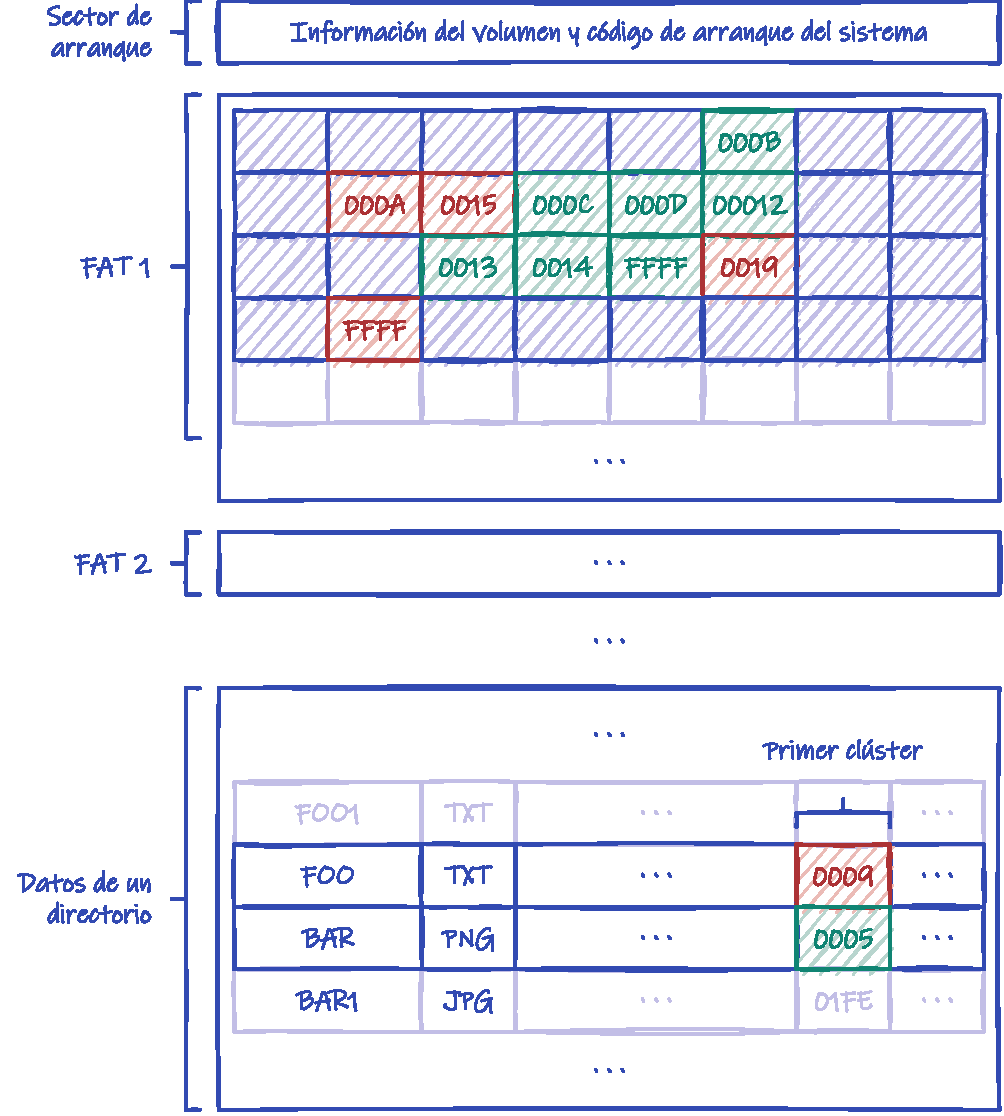
\includegraphics[width=0.8\textwidth]{media/C20_implemantación_sistema_de_archivos/estructura_fat.pdf}
\caption{Asignación enlazada en el sistema de archivos
FAT.}\label{fig-estructura-fat}
\end{figure}

Una de las ventajas de este esquema es que mejora el tiempo de los
accesos aleatorios a los archivos ---respecto a la asignación enlazada
convencional--- porque se puede conocer la ubicación de cualquier bloque
a partir de la información en la FAT, sin tener que leer todos los
bloques del archivo uno a uno.

\subsection{Asignación indexada}\label{_asignaciuxf3n_indexada}

{} El mecanismo de \textbf{asignación indexada} agrupa todos los
punteros de la asignación enlazada en una única ubicación: el
\textbf{bloque de índices}{}. Así se resuelve la falta de eficiencia de
la asignación enlazada convencional ---en ausencia de FAT--- cuando se
realizan accesos aleatorios.

En la \textbf{asignación indexada}:

\begin{itemize}
\item
  Cada archivo tiene su propio \textbf{bloque de índices}, que es un
  bloque del disco con una tabla con los números de los bloques del
  disco que contienen los datos del archivo.
\item
  La entrada i-ésima del bloque de índice contiene la dirección del
  bloque i-ésimo del archivo.
\item
  Cada entrada de directorio contiene la dirección del bloque de índices
  del archivo correspondiente.
\end{itemize}

Este mecanismo soporta el acceso aleatorio eficiente, además de no
sufrir el problema de la fragmentación externa. Sin embargo, también
tiene sus desventajas:

\begin{itemize}
\item
  Se pierde más espacio en los punteros que con el mecanismo de
  asignación enlazada, pues siempre hay que reservar un \textbf{bloque
  de índices} completo para cada archivo. Mientras que con la asignación
  enlazada, solo se pierde el espacio de los punteros que realmente es
  necesario utilizar.
\item
  Al diseñar el sistema de archivos debemos determinar el tamaño del
  \textbf{bloque de índices}.

  Por el inconveniente anterior y puesto que cada archivo debe tener un
  bloque de índices, ese bloque debe ser lo más pequeño posible para no
  perder espacio. Pero si es demasiado pequeño, no podrá almacenar
  suficientes punteros para un archivo de gran tamaño.
\end{itemize}

Entre los mecanismos que pueden utilizarse para resolver este último
problema están los siguientes:

\begin{itemize}
\item
  En el \textbf{esquema enlazado}{}, se enlazan los bloques de índices.

  Por ejemplo, se puede utilizar el último puntero del bloque de índices
  para apuntar al siguiente bloque de índices. Si dicho puntero tiene
  valor 0, entonces estamos en el último bloque de índices del archivo.
\item
  En el \textbf{índice multinivel}{}, los punteros del bloque de índices
  no señalan a los bloques del archivo, sino a un conjunto de bloques de
  índices de segundo nivel y estos, a su vez señalan, a los bloques del
  archivo. Esta técnica puede ampliarse utilizando un tercer o cuarto
  nivel, dependiendo del tamaño máximo de archivo que se desee.
\item
  En el \textbf{esquema combinado}{} las primeras entradas del bloque de
  índices apuntan directamente a los primeros bloques del archivo.
  Mientras que las siguientes entradas contiene punteros indirectos, que
  apunta a un conjunto de bloques de índices de segundo nivel. Después
  podría haber entradas que contienen punteros doblemente indirectos y
  luego entradas con punteros triplemente indirectos.
\end{itemize}

Para mejorar el rendimiento de los mecanismos de asignación indexados,
es muy común que el sistema operativo intente mantener los bloques de
índices en la memoria.

\begin{figure}
\centering
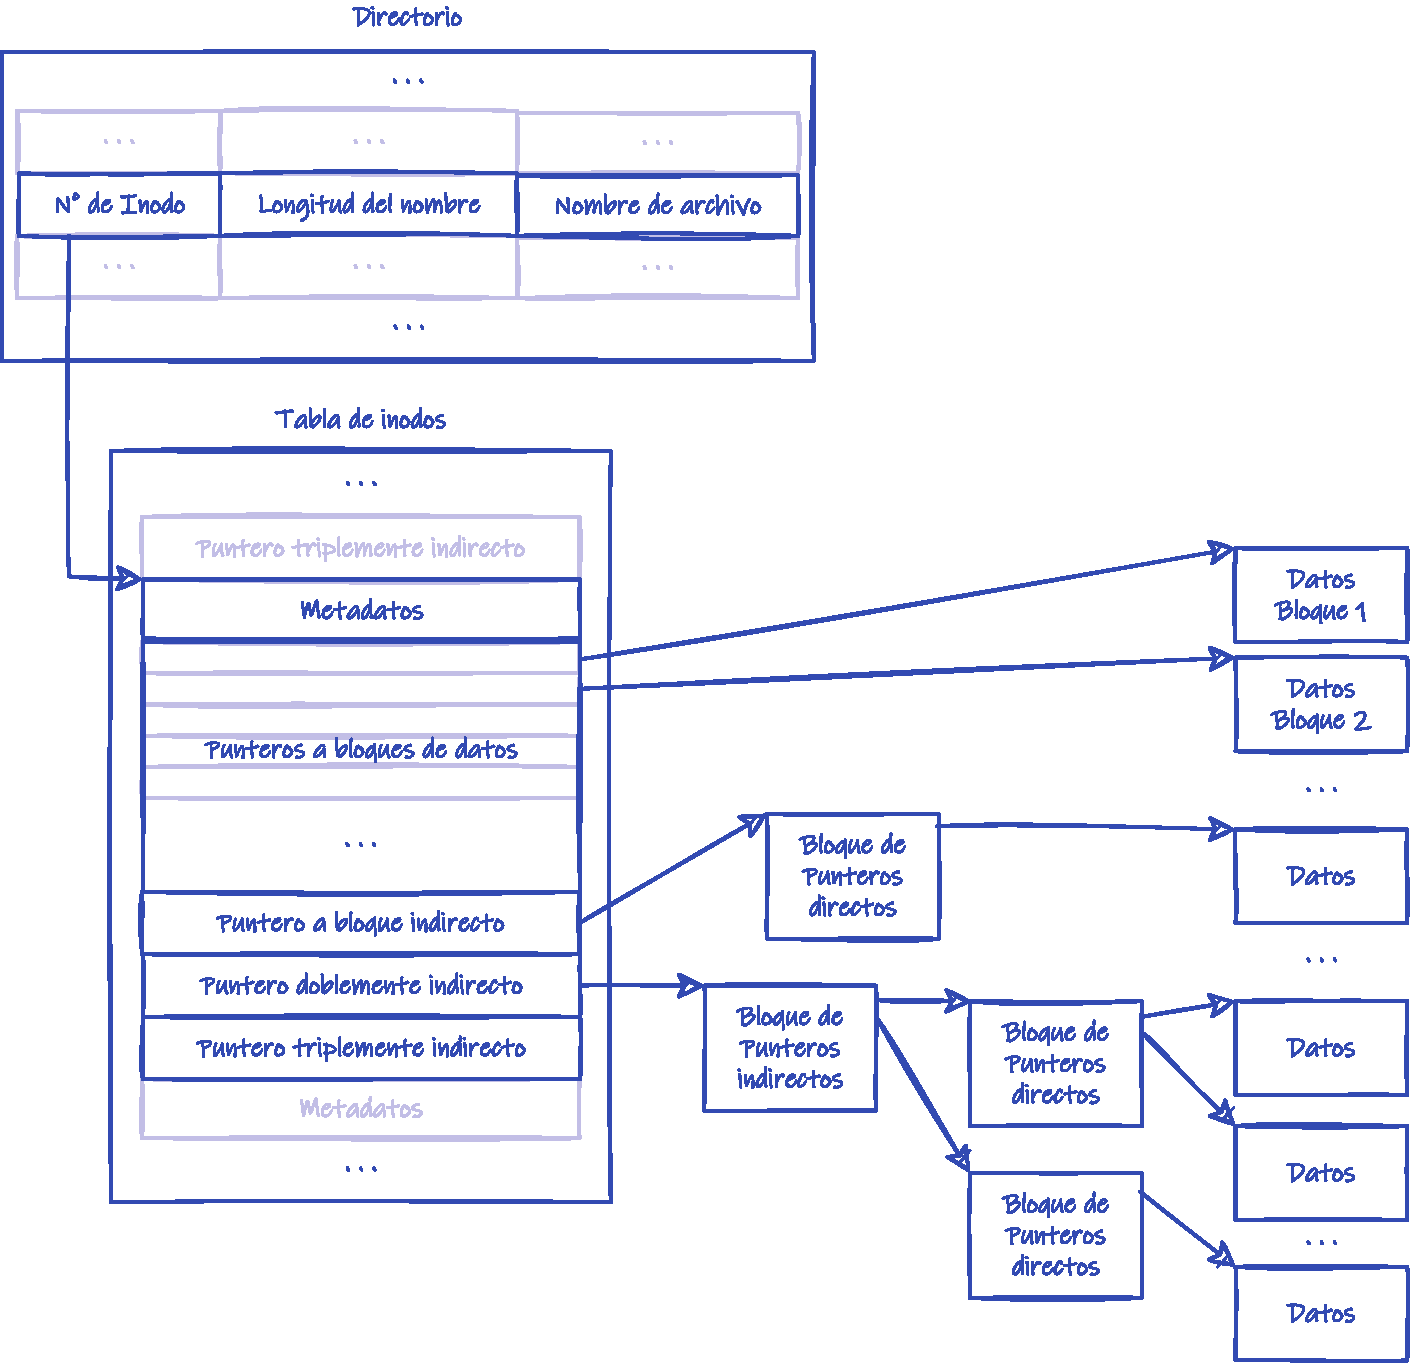
\includegraphics[width=0.8\textwidth]{media/C20_implemantación_sistema_de_archivos/asignación_ext2.pdf}
\caption{Asignación indexada combinada en el sistema de archivos
ext2.}\label{fig-asignaciuxf3n-ext2}
\end{figure}

Los sistemas de archivos \{ext2\} y \{ext3\} utilizan el mecanismo de
\textbf{asignación indexada} con \textbf{esquema combinado}.
Concretamente el mecanismo en \{ext2\} se implementa de la siguiente
manera:

\begin{itemize}
\item
  El disco se divide en múltiples grupos de bloques de disco.
\item
  En cada grupo, se utilizan los primeros bloques para almacenar una
  tabla de \textbf{inodos}{}. Estos \textbf{inodos} son los \textbf{FCB}
  de los archivos almacenados en el grupo.

  El resto de los bloques se utilizan para almacenar los datos de los
  archivos representados por los \textbf{inodos} del grupo.
\item
  Dentro de cada \textbf{inodo} ---entre otra información típica en un
  \textbf{FCB}--- se almacenan los punteros a los bloques del archivo,
  en lugar de utilizar un bloque de índices aparte.
\item
  Como se puede ver en la \hyperref[fig-asignaciuxf3n-ext2]{Asignación
  indexada combinada en el sistema de archivos ext2.}, los primeros 12
  punteros en el \textbf{inodo} son directos, seguidos de un puntero
  indirecto, un puntero doblemente indirecto y uno triplemente
  indirecto. Esto permite almacenar hasta 2\textsuperscript{64} bytes de
  información en cada archivo.
\end{itemize}

\section{Gestión del espacio libre}\label{_gestiuxf3n_del_espacio_libre}

Puesto que el espacio en disco es limitado, necesitamos poder reutilizar
el espacio de los archivos borrados. Para controlar el espacio libre en
el disco, el sistema de archivos mantiene una \textbf{lista de espacio
libre} que contiene todos los bloques de disco disponibles. Para crear
un archivo, se explora la \textbf{lista de espacio libre} hasta obtener
la cantidad de espacio requerida y se asigna ese espacio al nuevo
archivo.

A continuación estudiaremos las diferentes maneras de implementar esa
lista.

\subsection{Vector de bits}\label{_vector_de_bits}

La lista de espacio libre puede ser implementada como un \textbf{vector
de bits} o \textbf{mapa de bits}, donde cada bloque es representado por
un bit. Si el bloque está libre, el bit está a 1, mientras que si el
bloque está asignado, el bit está a 0.

Este enfoque es relativamente sencillo y eficiente, puesto que muchos
procesadores disponen de instrucciones para manipular bits, que pueden
utilizarse para obtener rápidamente el primer bloque libre. Por ejemplo,
la familia de procesadores \{x86\}, a partir del \{intel80386\}, tiene
instrucciones que devuelven la posición del primer bit a 1 en el valor
de un registro.

Sin embargo, leer el vector de bits, modificarlo y actualizarlo en disco
en cada ocasión, es tremendamente ineficiente. Por tanto, usar vectores
de bits es ineficiente, a menos que se mantenga el vector completo en la
memoria principal, escribiéndose ocasionalmente en el disco.

Esto último puede ser imposible para los discos de gran tamaño, en
función de la cantidad de memoria principal. Por ejemplo, un disco de 40
GiB con bloques de 512 bytes necesitará un mapa de bits de más de 10
MiB, lo que no es un gran requisito para un sistema moderno, pero sí lo
era hace dos décadas.

El sistema de archivo NTFS y la familia \emph{extended filesystem} ---es
decir, \{ext\}, \{ext2\}, \{ext3\} y \{ext4--- utilizan mapas de bits,
tanto para gestionar los bloques de datos libres como las entradas
disponibles en la tabla de \textbf{inodos}.

\subsection{Lista enlazada}\label{_lista_enlazada}

Otra técnica consiste en enlazar todos los bloques de disco libres. Para
eso se puede guardar un puntero al primer bloque libre en una ubicación
especial del disco y que ese bloque contenga un puntero al siguiente
bloque libre del disco. El segundo bloque contenga un puntero al tercer
bloque libre, y así sucesivamente.

El inconveniente es que recorrer la lista no resulta eficiente, pues
tenemos que leer cada bloque para conocer la dirección del siguiente
bloque libre en disco. Sin embargo, debemos tener en cuenta que no es
frecuente tener que recorrer la lista de espacio libre completa porque,
por lo general, basta con encontrar el primer bloque libre para asignar
el espacio.

Los sistemas de archivos \{fat\} incorporan el control de bloques libres
dentro de la \textbf{tabla de asignación de archivos} guardando un 0 en
las entradas de los \textbf{clústeres} libres, por lo que no se necesita
ningún método adicional.

\subsection{Agrupamiento}\label{_agrupamiento}

Una modificación de la técnica basada en la lista enlazada consiste en
almacenar las direcciones de \emph{N} bloques libres en el primer bloque
libre. Los primeros \emph{N --- 1} de esos bloques estarían realmente
libres, pero el último de ellos apuntaría a otro bloque con \emph{N}
bloques libres. Así podrían localizarse rápidamente las direcciones de
un gran número de bloques libres, lo cual mejora la eficiencia respecto
a la técnica de lista enlazada.

\subsection{Recuento}\label{_recuento}

Generalmente los bloques son asignados o liberados en bloques contiguos,
especialmente si el espacio es asignado mediante asignación contigua o
en \textbf{extensiones} o \textbf{clústeres}. Esto puede ser aprovechado
para mantener una lista donde cada entrada almacena la dirección del
primer bloque de un conjunto de bloques libres contiguo, así como el
número de bloques del conjunto.

Por ejemplo, el sistema de archivos \{xfs\} utiliza un árbol B+ para
almacenar las direcciones de las extensiones de bloques libres y
mantenerlas ordenadas por el tamaño de la extensión a la que apuntan.
Así el sistema operativo puede localizar rápidamente el espacio libre
necesario para satisfacer una necesidad concreta.

\section{Sistemas de archivos
virtuales}\label{_sistemas_de_archivos_virtuales}

En el \hyperref[_montaje_de_sistemas_de_archivos]{???} vimos cómo el
sistema operativo \textbf{monta} sistemas de archivos de tal forma que
aparenten estar integrados en una única estructura de directorios,
permitiendo a los usuarios moverse de forma transparente entre distintos
dispositivos y tipos de sistemas de archivos. Para hacerlo, un sistema
operativo moderno debe ser capaz de soportar de manera eficiente
distintos tipos de sistemas de archivos, ocultando sus diferencias de
cara a los usuarios.

Un método para implementar múltiples tipos de sistemas de archivos
consiste en escribir diferentes rutinas de acceso, manipulación y
gestión ---de los directorios y archivos--- para cada uno de los tipos
de sistema de archivo existentes. Sin embargo, en lugar de esta
solución, la mayoría de los sistemas operativos utilizan técnicas de
programación orientada a objetos para implementar diferentes tipos de
sistemas de archivos detrás de una misma interfaz de programación. Es
decir, se utilizan estructuras de datos y procedimientos comunes para
separar las llamadas al sistema de los detalles de su implementación
real, para cada uno de los sistemas de archivos.

La implementación de un sistema de archivos está compuesta de tres
niveles fundamentales: la \textbf{interfaz del sistema de archivos}, el
\textbf{sistema de archivos virtual} y, finalmente, la implementación
real del sistema de archivos.

\subsection{Interfaz del sistema de
archivos}\label{_interfaz_del_sistema_de_archivos}

{} El primer nivel es la \textbf{interfaz del sistema de archivos}, a la
que acceden los desarrolladores a través de las llamadas al sistema. En
sistemas POSIX, estamos hablando de las llamadas \{linux\_open\},
\{linux\_read\}, \{linux\_write\} y \{linux\_close\}, entre otras. Y de
los descriptores de archivos con los que se identifican los archivos
abiertos.

Esta interfaz es la misma sea cual sea el sistema de archivos al que se
esté intentando acceder.

\subsection{Sistema de archivos
virtual}\label{_sistema_de_archivos_virtual}

{} El segundo nivel es la interfaz del \textbf{sistema de archivos
virtual} o \textbf{{}VFS} (\emph{Virtual File System}). Este nivel es
utilizado por el anterior para atender las peticiones realizadas.

Describe operaciones genéricas sobre cualquier sistema de archivos y
estructuras genéricas. Por ejemplo, el \textbf{FCB virtual}{}, que
identifica de forma unívoca a cada archivo o directorio en uso en todo
el sistema, dando acceso a sus metadatos.

En Linux el \textbf{FCB virtual} se denomina \textbf{{}vnodo}. El
\textbf{vnodo} de un archivo lo identifica de forma unívoca en todo el
sistema, incluso diferenciando archivos en sistemas de archivos
diferentes. Mientras que el \textbf{inodo} es un detalle de la
implementación real del sistema de archivos, por lo que solo es único
dentro del mismo sistema de archivos.

Este nivel cumple con dos importantes funciones:

\begin{itemize}
\item
  Separa las operaciones genéricas sobre el sistema de archivos con
  respecto a su implementación.

  \textbf{VFS} define una interfaz muy clara y común para todos los
  sistemas de archivos. De esta interfaz existirán diversas
  implementaciones en el mismo sistema, una para cada sistema de
  archivos diferente.
\item
  Proporcionar un mecanismo para acceder de forma coherente a los
  archivos a través de la red.

  Una implementación de \textbf{VFS} no tiene que estar limitada
  exclusivamente a ofrecer acceso a archivos en dispositivos conectados
  físicamente al sistema. Las operaciones de la interfaz \textbf{VFS}
  pueden implementarse de tal forma que usen un protocolo de acceso a
  algún servidor de archivos conectado a la red.
\end{itemize}

\subsection{Implementación del sistema de
archivos}\label{_implementaciuxf3n_del_sistema_de_archivos}

El tercer nivel es donde se implementa cada tipo de sistema de archivos
o los distintos protocolos de los servidores de archivos en la red. La
interfaz \textbf{VFS} recurre a la implementación correspondiente para
cada tipo de sistema de archivos, para satisfacer las solicitudes de los
niveles superiores.

Así, por ejemplo, un \{linux\_read\} puede implicar que se tenga que
recuperar el \textbf{vnodo} del archivo involucrado desde la tabla de
archivos abiertos, usando el descriptor de archivo indicado en la
llamada al sistema. Después, se invoca la operación \textbf{VFS}
\texttt{read()} sobre el \textbf{vnodo}, en la implementación concreta
de \textbf{VFS} según el tipo de sistema de archivos involucrado. Será
esa implementación quien extraiga del \textbf{vnodo} la información
necesaria ---por ejemplo, el \textbf{inodo} real del archivo en el
sistema de archivos--- para llevar a cabo la operación indicada, según
las especificidades del sistema de archivos.

\section{Planificación de disco}\label{_planificaciuxf3n_de_disco}

Como ya hemos comentado, es responsabilidad del sistema operativo usar
los recursos del hardware de forma eficiente. Eso incluye planificar los
procesos en la CPU para conseguir el mínimo tiempo de espera que sea
posible o aprovechar de la mejor forma la memoria principal disponible
para atender la demanda de los distintos procesos al mismo tiempo; pero
también, intentar obtener el menor tiempo de acceso y el mayor ancho de
banda posible en el acceso a los discos.

\subsection{Rendimiento del acceso a
disco}\label{_rendimiento_del_acceso_a_disco}

En un disco duro magnético el \textbf{tiempo de acceso al disco}{}
\emph{T\textsuperscript{d}} viene determinado por el \textbf{tiempo de
búsqueda} \emph{T\textsuperscript{b}} y la \textbf{latencia rotacional}
\emph{T\textsuperscript{r}}:

\[T_d=T_b+T_r\]

El \textbf{tiempo de búsqueda}{} \emph{T\textsuperscript{b}} es el
tiempo que se tarda en mover el brazo del disco hasta el cilindro
deseado. Mientras que la \textbf{latencia rotacional}{}
\emph{T\textsuperscript{r}} es el tiempo que hay que esperar para que el
disco gira hasta que la cabeza llegue al sector deseado del cilindro.
Por lo tanto, el \textbf{tiempo de acceso al disco} es menor cuando se
realizan accesos consecutivos a sectores físicamente próximos que cuando
están dispersos por todo el disco.

El \textbf{{}ancho de banda} o \textbf{tasa de transferencia}{} del
disco es el total de bytes transferidos en una petición dividida por el
tiempo total que transcurre desde la primera solicitud de servicio hasta
el final de la última transferencia, con la que se termina de atender la
petición. Al considerar todo el tiempo necesario para atender la
petición, a más \textbf{tiempo de acceso al disco} menor es el
\textbf{ancho de banda}.

En los dispositivos de almacenamiento basados en memorias de estado
sólido (véase el \hyperref[_memorias_de_estado_suxf3lido]{???}) el
tiempo de acceso viene determinado por las características de la memoria
---entre otros factores--- lo que hace que las diferencias entre accesos
secuenciales y accesos aleatorios sean mucho menos significativas.

\subsection{Cola de E/S al disco}\label{_cola_de_es_al_disco}

{} Cuando se solicita una operación de E/S sobre el almacenamiento, si
la controladora y la unidad de disco están desocupadas, el sistema
operativo puede atender la petición sobre la marcha. Pero si están
ocupadas, el sistema operativo almacena la solicitud en una cola de
peticiones pendientes. Cuando se resuelve una solicitud, el sistema
operativo escoge otra de la cola y se comunica con el hardware para
programar la siguiente petición. La cuestión es ¿cuál es el orden
adecuado para escoger la peticiones de E/S de la cola, si se quiere
acceder al disco de la forma más eficaz posible?

\subsection{Planificación FCFS}\label{_planificaciuxf3n_fcfs}

{} En la planificación \textbf{{}FCFS} (\emph{First Come, First Served})
o \textbf{primero que llega, primero servido} la cola de E/S al disco es
FIFO. Es decir, que las solicitudes se atienden en orden de llegada.

Es el algoritmo de planificación más simple y es equitativo, en sentido
de que atiende a todos los procesos por igual. Pero, lamentablemente, no
proporciona el servicio más rápido en discos duros magnéticos, donde
interesa mover el brazo del disco lo menos posible.

En Linux el \textbf{FCFS} es actualmente denominado \textbf{NOOP}. Se
suele utilizar en los discos basados en memorias de estado sólido, donde
reordenar las solicitudes no proporciona una mejora significativa del
rendimiento, o cuando se utilizan controladoras de disco inteligentes
que pueden reordenar las solicitudes según su propio criterio.

\subsection{Planificación SSTF}\label{_planificaciuxf3n_sstf}

{} En la planificación \textbf{{}SSTF} (\emph{Sortest} \emph{Seek Time
First}) o algoritmo de \textbf{tiempo de búsqueda más corto}, de toda
cola se selecciona la solicitud con el menor \textbf{tiempo de búsqueda}
desde la posición actual de la cabeza. Este algoritmo de planificación
primero da servicio a las solicitudes cercanas a la posición actual de
la cabeza, antes de alejarse para dar servicio a otras solicitudes, dado
que el \textbf{tiempo de búsqueda} se incrementa a medida que lo hace el
número de cilindros que es necesario recorrer para llegar a una posición
dada.

Aun así, la solución no es óptima, dado que puede provocar inanición de
algunas solicitudes, si van llegando constantemente nuevas solicitudes
sobre regiones cercanas a donde está actualmente la cabeza del disco.

\subsection{Planificación SCAN y
C-SCAN}\label{_planificaciuxf3n_scan_y_c_scan}

{} {} En la planificación \textbf{{}SCAN}, algoritmo de
\textbf{exploración} o del \textbf{ascensor}, el brazo del disco
comienza en un extremo del disco y se mueve hacia el otro, atendiendo
solicitudes a medida que pasa por cada cilindro, hasta llegar al otro
extremo del disco. En el otro extremo, la dirección de movimiento de la
cabeza se invierte para recorrer el disco en sentido inverso, repitiendo
el proceso.

Suponiendo que las solicitudes se distribuyen de forma uniforme a lo
largo del disco, es de suponer que cuando se llega a un extremo ---justo
antes de volver--- la cantidad de solicitudes en dicho extremo será
notablemente menor que dónde comenzó el barrido que acaba de terminar.
Entonces ¿por qué no volver a empezar desde ese extremo?

A la variante del \textbf{SCAN} que cuando llega a un extremo vuelve al
inicio, para volver a barrer desde allí, sin atender ninguna solicitud
por el camino, se la denomina \textbf{{}C-SCAN} ---de \emph{Circula
SCAN}---. Con esta variante el tiempo que tiene que esperar una
solicitud para ser atendida es más uniforme que con el algoritmo
\textbf{SCAN} original.

\subsection{Planificación LOOK y
C-LOOK}\label{_planificaciuxf3n_look_y_c_look}

{} {} En teoría los algoritmos \textbf{SCAN} y \textbf{C-SCAN} hacen que
el brazo recorra los cilindros del primero al último, pero normalmente
no se suelen implementar así.

Por lo general, cuando en el recorrido del brazo, tras atender una
solicitud, se descubre que ya no hay más solicitudes siguiendo la misma
dirección, el brazo invierte la dirección sin llegar hasta el extremo
del disco.

A estas variantes de \textbf{SCAN} y \textbf{C-SCAN} se las denomina
\textbf{(LOOK)} y \textbf{(C-LOOK)}, respectivamente.

Linux utilizó \textbf{C-LOOK}, bajo el nombre de
\textbf{\emph{elevator}}, como planificador de E/S de disco hasta Linux
2.6.

\subsection{Planificación N-Step-SCAN, N-Step-LOOK y
F-SCAN}\label{_planificaciuxf3n_n_step_scan_n_step_look_y_f_scan}

{} {} {} Los algoritmos \textbf{{}N-Step-SCAN} y \textbf{{}N-Step-LOOK}
son variantes de los algoritmos \textbf{SCAN} y \textbf{LOOK},
respectivamente; donde se limita a \emph{N} el número de solicitudes que
se atenderán en cada barrido del brazo del disco. Estos algoritmos
funcionan de la siguiente manera:

\begin{enumerate}
\def\labelenumi{\arabic{enumi}.}
\item
  Se utiliza una cola con espacio para \emph{N} solicitudes pendientes,
  que se van atendiendo mientras el brazo barre el disco.
\item
  Mientras tanto, todas las nuevas solicitudes se incorporan a una cola
  diferente.
\item
  Cuando el brazo termina el barrido y las \emph{N} primeras solicitudes
  han sido atendidas, el planificador toma otras \emph{N} solicitudes de
  la segunda cola y las introduce en la primera para repetir el proceso.
\end{enumerate}

Si en lugar de copiar \emph{N} peticiones de la segunda a la primera
cola, se copian todas las solicitudes pendientes, el algoritmo se
denomina \textbf{{}F-SCAN}.

Estos algoritmos previenen un problema denominado \textbf{{}rigidez del
brazo} ---o \emph{arm stickiness}, en inglés--- a diferencia de los
algoritmos SSTF, SCAN, C-SCAN, LOOK y C-LOOK, que no lo hacen. El
término \textbf{rigidez del brazo} hace referencia a cuando hay un flujo
continuo de solicitudes para el mismo cilindro, esto hace que con los
algoritmos vistos hasta ahora, el brazo no avance por los cilindros
hasta llegar al otro extremo. Como \textbf{F-SCAN}, \textbf{N-Step-SCAN}
y \textbf{N-Step-LOOK} separan las solicitudes en dos colas ---haciendo
que las nuevas tengan que esperar--- el brazo siempre continúa su
barrido hacia el extremo del disco.

\subsection{Planificación CFQ}\label{_planificaciuxf3n_cfq}

{} El planificador \textbf{{}CFQ} (\emph{Completely Fair Queuing}) se
diseñó para compartir de forma equitativa el \textbf{ancho de banda}
entre todos los procesos que solicitan acceso al disco. Fue utilizado
por defecto en muchas distribuciones de Linux hasta la versión 5.0 del
núcleo y funciona de la siguiente manera:

\begin{itemize}
\item
  \textbf{CFQ} mantiene una cola de solicitudes para cada proceso y en
  ella inserta las solicitudes síncronas de E/S. Cada cola tiene una
  ventana de tiempo ---o \textbf{cuanto}--- para acceder al disco. La
  longitud del \textbf{cuanto} y el tamaño máximo de cada cola dependen
  de la prioridad de E/S que tenga el proceso.
\end{itemize}

Las solicitudes síncronas de E/S son aquellas que hacen que el proceso
permanezca en estado \textbf{esperando} hasta que se resuelve la
petición. Por ejemplo, las operaciones de lectura bloqueantes, como
ocurre por defecto con \{linux\_read\}. Mientras que las solicitudes
asíncronas son las que permiten que el proceso continúe su ejecución en
la CPU mientras se atiende la petición. Como las escrituras con
\{linux\_write\}.

\begin{itemize}
\item
  \textbf{CFQ} mantiene una cola de solicitudes por cada prioridad de
  E/S, donde se insertan las solicitudes asíncronas de todos los
  procesos. Una solicitud asíncrona se inserta en una cola u otra según
  la prioridad del proceso que la generó.
\item
  Usando el algoritmo \textbf{\emph{round-robin}}, el planificador
  \textbf{CFQ} recorre las colas y extrae de ellas las solicitudes
  durante el tiempo marcado por el cuanto de cada cola. Las solicitudes
  extraídas se insertan en la cola de E/S al disco, donde se ordenan
  para minimizar el \textbf{tiempo de búsqueda}, antes de ser enviadas
  al dispositivo.
\end{itemize}

Actualmente, los planificadores \textbf{CFS} y \textbf{NOOP} se
consideran obsoletos. En su lugar el planificador por defecto en Linux
para SSD y discos duros es \textbf{mq-deadline} ---una adaptación del
planificador
\href{https://en.wikipedia.org/wiki/Deadline_scheduler}{deadline},
también obsoleto---. Mientras que para dispositivos NVM Express se
utiliza \textbf{NONE}, que básicamente desactiva la planificación de la
E/S de disco.

Otros planificadores disponibles actualmente son
\href{https://algo.ing.unimo.it/people/paolo/disk_sched/}{BFQ}
---diseñado para minimizar la latencia--- y Kyber.
